\documentclass{article}
\usepackage[latin1]{inputenc}
\usepackage{amsmath}
\usepackage{amsfonts}
\usepackage{amssymb}
\usepackage{graphicx}
\usepackage{hyperref}
\usepackage{pgfplots}
\begin{document}
	\begin{figure}
		\centering
		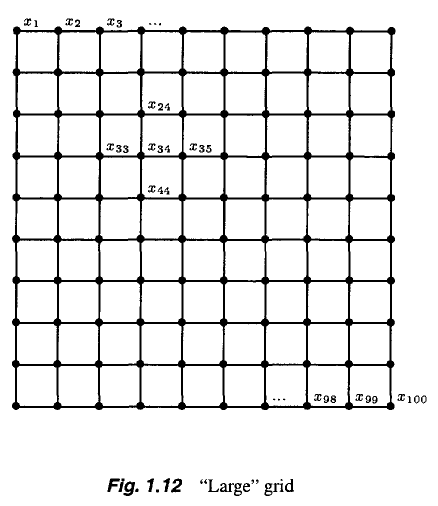
\includegraphics[width=0.7\linewidth]{C:/github/sandbox/books/FundamentalsMatrixComputations/figure112}
	\end{figure}
	Exercise 1.5.11\\
	\\
	As in Exercise 1.5.4, consider the banded system of equations arising from an $m \times m$ network of nodes like Figure 1.12 but larger, with the nodes numbered by rows, as in Figure 1.12.\\
	\\ 
	(a) For the case m = 100 (for which $n = 10^4$) calculate the cost of solving the system $Ax = b$ (Cholesky decomposition plus forward and back substitution) with and without exploiting the band structure. Show that exploiting the band structure cuts the flop count by a factor of several thousand. Show that if only the semiband is stored, the storage space required is only about 1% of what 
	would be required to store the matrix naively.\\
	\\
	(b) Repeat part (a) with m = 1000. 
	\\
	Answers:\\
	\\		
	(a) Any link can theorically be linked to any other node, on a $100 \times 100$ this means we have a $n=10^4$ matrix.\\
	\\
	\\
	\\	
	Solving this system using naive Cholesky method will cost:\\
	Cholesky ($n^3/3$):$\frac{(10^4)^3}{3}=\frac{10^{12}}{3}$\\
	Foward Substitution ($n^2$):$(10^4)^2=10^8$\\
	Backward Substitution ($n^2$):$(10^4)^2=10^8$\\
	Total:\\
	\begin{align*}
		\frac{10^{12}}{3} + 10^8 + 10^8 = \frac{10^{12}}{3} + 2*10^8 \approx 10^{12}
	\end{align*}
	\\
	Solving using Banded-Matrix with band $s=100$:\\
	Banded Cholesky ($ns^2$): $ 10^4 * 100^2 = 10^4 * (10^2)^2 = 10^4 * 10^4 = 10^8  $\\
	Foward Substitution ($2ns$):$ 2*10^{4}*100 = 2*10^{4}*10^{2} = 2*10^{4}*10^{2} = 2*10^6$\\
	Backward Substitution ($2ns$):$ 2*10^{4}*100 = 2*10^{4}*10^{2} = 2*10^{4}*10^{2} = 2*10^6$\\
	\\
	Total:\\
	\begin{align*}
		10^8 + 2*10^6 + 2*10^6 = 10^8 + 4*10^6 \approx 10^{8}
	\end{align*}
	\\
	Using a Band optimized algorithms we gain:\\
	\begin{align*}
		\frac{10^8}{10^{12}} = 	\frac{10^8}{10^{8}*10^{4}} = \frac{1}{10^{4}} = 0.01 \%
	\end{align*}
	$1$ghz is $1.000.000.000$ of cycles per second, or $10^9$ cycles per second. In the naive scenario we are going to make $1^12$ operations. If we average that every operation takes:zz
	1 cycle per operation (ASM operation)\\
	50 cycles per operation (memory access of all variables)\\
	\\
	Which will be approximated to 50 cycles per operation.\\
	The naive approach.\\
	\begin{align*}
		10^{12} * 50 &=	10^{12} * 5*10 \text{ cycles}\\
		&= 5*10^{13} \text{ cycles}\\
		&= 5*10^{5}*10^{9} \text{ cycles}\\
		&= 5*10^{5}*10^{9} \text{ cycles} * \frac{1 \text{ sec}}{10^9 \text{ cycles}}\\
		&= 5*10^{5}*10^{9} \text{ cycles} * \frac{1 \text{ sec}}{10^9 \text{ cycles}}\\		
		&= 5*10^{5} \text{ sec}\\		
	\end{align*}
	The naive approach.\\
	\begin{align*}
	10^{12} * 50 &=	10^{12} * 5*10 \text{ cycles}\\
	&= 5*10^{13} \text{ cycles}\\
	&= 5*10^{5}*10^{9} \text{ cycles}\\
	&= 5*10^{5}*10^{9} \text{ cycles} * \frac{1 \text{ sec}}{10^9 \text{ cycles}}\\
	&= 5*10^{5}*10^{9} \text{ cycles} * \frac{1 \text{ sec}}{10^9 \text{ cycles}}\\		
	&= 5*10^{5} \text{ sec}\\		
	&\approx 8333 \text{ min}\\		
	&\approx 138 \text{ hours}\\			
	&\approx 6 \text{ days}\\	
	\end{align*}
	The banded optimized approach:\\
	\begin{align*}
	10^{8} * 50 &=	10^{8} * 5*10 \text{ cycles}\\
	&= 5*10^{9} \text{ cycles}\\
	&= 5*10^{9} \text{ cycles} * \frac{1 \text{ sec}}{10^9 \text{ cycles}}\\
	&= 5 \text{ sec}\\		
	\end{align*}
	\\
	(b) If we increase $m=1000$, $n$ will be $n=10^6$.\\\\
	Solving this system using naive Cholesky method will cost:\\
	Cholesky ($n^3/3$):$\frac{(10^6)^3}{3}=\frac{10^{18}}{3}$\\
	Foward Substitution ($n^2$):$(10^6)^2=10^{12}$\\
	Backward Substitution ($n^2$):$(10^6)^2=10^{12}$\\\\
	Solving using Banded-Matrix with band $s=1000$:\\
	Banded Cholesky ($ns^2$): $ 10^6 * 1000^2 = 10^6 * (10^3)^2 = 10^6 * 10^9 = 10^{15} $\\
	Foward Substitution ($2ns$):$ 2*10^{6}*1000 = 2*10^{6}*10^{3} = 2*10^9$\\
	Backward Substitution ($2ns$):$ 2*10^{6}*1000 = 2*10^{6}*10^{3} = 2*10^9$\\
	\\
	\begin{align*}
		\frac{10^{15}}{10^{18}} = \frac{10^{15}}{10^{15}*10^{3}} = \frac{1}{10^3} = 0.1 \%
	\end{align*}
\end{document}